\documentclass[12pt,english]{article}\usepackage[]{graphicx}\usepackage[]{xcolor}
% maxwidth is the original width if it is less than linewidth
% otherwise use linewidth (to make sure the graphics do not exceed the margin)
\makeatletter
\def\maxwidth{ %
  \ifdim\Gin@nat@width>\linewidth
    \linewidth
  \else
    \Gin@nat@width
  \fi
}
\makeatother

\definecolor{fgcolor}{rgb}{0.345, 0.345, 0.345}
\newcommand{\hlnum}[1]{\textcolor[rgb]{0.686,0.059,0.569}{#1}}%
\newcommand{\hlsng}[1]{\textcolor[rgb]{0.192,0.494,0.8}{#1}}%
\newcommand{\hlcom}[1]{\textcolor[rgb]{0.678,0.584,0.686}{\textit{#1}}}%
\newcommand{\hlopt}[1]{\textcolor[rgb]{0,0,0}{#1}}%
\newcommand{\hldef}[1]{\textcolor[rgb]{0.345,0.345,0.345}{#1}}%
\newcommand{\hlkwa}[1]{\textcolor[rgb]{0.161,0.373,0.58}{\textbf{#1}}}%
\newcommand{\hlkwb}[1]{\textcolor[rgb]{0.69,0.353,0.396}{#1}}%
\newcommand{\hlkwc}[1]{\textcolor[rgb]{0.333,0.667,0.333}{#1}}%
\newcommand{\hlkwd}[1]{\textcolor[rgb]{0.737,0.353,0.396}{\textbf{#1}}}%
\let\hlipl\hlkwb

\usepackage{framed}
\makeatletter
\newenvironment{kframe}{%
 \def\at@end@of@kframe{}%
 \ifinner\ifhmode%
  \def\at@end@of@kframe{\end{minipage}}%
  \begin{minipage}{\columnwidth}%
 \fi\fi%
 \def\FrameCommand##1{\hskip\@totalleftmargin \hskip-\fboxsep
 \colorbox{shadecolor}{##1}\hskip-\fboxsep
     % There is no \\@totalrightmargin, so:
     \hskip-\linewidth \hskip-\@totalleftmargin \hskip\columnwidth}%
 \MakeFramed {\advance\hsize-\width
   \@totalleftmargin\z@ \linewidth\hsize
   \@setminipage}}%
 {\par\unskip\endMakeFramed%
 \at@end@of@kframe}
\makeatother

\definecolor{shadecolor}{rgb}{.97, .97, .97}
\definecolor{messagecolor}{rgb}{0, 0, 0}
\definecolor{warningcolor}{rgb}{1, 0, 1}
\definecolor{errorcolor}{rgb}{1, 0, 0}
\newenvironment{knitrout}{}{} % an empty environment to be redefined in TeX

\usepackage{alltt}
\usepackage{mypreamble,myRpreamble,enumitem}
\IfFileExists{upquote.sty}{\usepackage{upquote}}{}
\begin{document}
{\bf Arkaraj Mukherjee \\ Worksheet 12}
\begin{knitrout}
\definecolor{shadecolor}{rgb}{0.969, 0.969, 0.969}\color{fgcolor}\begin{kframe}
\begin{alltt}
\hlkwd{library}\hldef{(}\hlsng{"tidyverse"}\hldef{);}
\end{alltt}


{\ttfamily\noindent\itshape\color{messagecolor}{\#\# -- Attaching core tidyverse packages ---------------------------------------- tidyverse 2.0.0 --\\\#\# v dplyr \ \ \ \ 1.2.0 \ \ \ \ v readr \ \ \ \ 2.1.6\\\#\# v forcats \ \ 1.0.1 \ \ \ \ v stringr \ \ 1.6.0\\\#\# v ggplot2 \ \ 4.0.2 \ \ \ \ v tibble \ \ \ 3.3.1\\\#\# v lubridate 1.9.5 \ \ \ \ v tidyr \ \ \ \ 1.3.2\\\#\# v purrr \ \ \ \ 1.2.1 \ \ \ \ \\\#\# -- Conflicts ---------------------------------------------------------- tidyverse\_conflicts() --\\\#\# x dplyr::filter() masks stats::filter()\\\#\# x dplyr::lag() \ \ \ masks stats::lag()\\\#\# i Use the conflicted package (<http://conflicted.r-lib.org/>) to force all conflicts to become errors}}\end{kframe}
\end{knitrout}

\begin{enumerate}[label=\arabic*.]
\item \begin{enumerate}[label=(\alph*)]
		\item We have that 
			\[
				L(\beta_1)=\prod_{i=1}^{15}\prod_{j=1}^{15} \frac{e^{\beta_1(x_i-x_j)^2}}{1+e^{\beta_1(x_i-x_j)^2}}
			\]
		\item 
\begin{knitrout}
\definecolor{shadecolor}{rgb}{0.969, 0.969, 0.969}\color{fgcolor}\begin{kframe}
\begin{alltt}
\hldef{x} \hlkwb{=} \hlkwd{c}\hldef{(}\hlnum{11}\hldef{,}\hlnum{9}\hldef{,}\hlnum{12}\hldef{,}\hlnum{9}\hldef{,}\hlnum{10}\hldef{,}\hlnum{11}\hldef{,}\hlnum{7}\hldef{,}\hlnum{9}\hldef{,}\hlnum{10}\hldef{,}\hlnum{9}\hldef{,}\hlnum{10}\hldef{,}\hlnum{10}\hldef{,}\hlnum{9}\hldef{,}\hlnum{11}\hldef{,}\hlnum{8}\hldef{)}
\hlcom{# we make the adjacency matrix first}
\hldef{G} \hlkwb{=} \hlkwd{matrix}\hldef{(}\hlkwc{data}\hldef{=}\hlnum{0}\hldef{,}\hlkwc{nrow}\hldef{=}\hlnum{15}\hldef{,}\hlkwc{ncol}\hldef{=}\hlnum{15}\hldef{)}
\hldef{G[}\hlnum{1}\hldef{,}\hlkwd{c}\hldef{(}\hlnum{6}\hldef{,}\hlnum{9}\hldef{)]}\hlkwb{=}\hlnum{1}
\hldef{G[}\hlnum{2}\hldef{,}\hlkwd{c}\hldef{(}\hlnum{8}\hldef{,}\hlnum{12}\hldef{)]}\hlkwb{=}\hlnum{1}
\hldef{G[}\hlnum{4}\hldef{,}\hlnum{10}\hldef{]}\hlkwb{=}\hlnum{1}
\hldef{G[}\hlnum{5}\hldef{,}\hlnum{9}\hldef{]}\hlkwb{=}\hlnum{1}
\hldef{G[}\hlnum{6}\hldef{,}\hlnum{14}\hldef{]}\hlkwb{=}\hlnum{1}
\hldef{G[}\hlnum{7}\hldef{,}\hlnum{15}\hldef{]}\hlkwb{=}\hlnum{1}
\hldef{G[}\hlnum{8}\hldef{,}\hlkwd{c}\hldef{(}\hlnum{10}\hldef{,}\hlnum{11}\hldef{,}\hlnum{15}\hldef{)]}\hlkwb{=}\hlnum{1}
\hldef{G[}\hlnum{9}\hldef{,}\hlnum{11}\hldef{]}\hlkwb{=}\hlnum{1}
\hldef{G[}\hlnum{13}\hldef{,}\hlnum{15}\hldef{]}\hlkwb{=}\hlnum{1}
\hldef{G} \hlkwb{=} \hldef{G} \hlopt{+} \hlkwd{t}\hldef{(G)}
\hldef{Prob} \hlkwb{=} \hlkwa{function}\hldef{(}\hlkwc{x}\hldef{,}\hlkwc{i}\hldef{,}\hlkwc{j}\hldef{,}\hlkwc{beta}\hldef{) \{}
\hlkwd{exp}\hldef{(beta}\hlopt{*}\hldef{(x[i]}\hlopt{-}\hldef{x[j])}\hlopt{^}\hlnum{2}\hldef{)}\hlopt{/}\hldef{(}\hlnum{1}\hlopt{+}\hlkwd{exp}\hldef{(beta}\hlopt{*}\hldef{(x[i]}\hlopt{-}\hldef{x[j])}\hlopt{^}\hlnum{2}\hldef{))}
\hldef{\}}
\hldef{init_L} \hlkwb{=} \hlkwa{function}\hldef{(}\hlkwc{x}\hldef{,}\hlkwc{G}\hldef{,}\hlkwc{beta}\hldef{) \{}
        \hldef{P} \hlkwb{=} \hlnum{1}
        \hlkwa{for}\hldef{(i} \hlkwa{in} \hlnum{1}\hlopt{:}\hlkwd{nrow}\hldef{(G)) \{}
                \hlkwa{for}\hldef{(j} \hlkwa{in} \hlnum{1}\hlopt{:}\hlkwd{ncol}\hldef{(G)) \{}
                        \hlkwa{if}\hldef{( G[i,j]} \hlopt{==} \hlnum{1} \hldef{) \{P} \hlkwb{=} \hldef{P} \hlopt{*} \hlkwd{Prob}\hldef{(x,i,j,beta)\}}
                        \hlkwa{if}\hldef{( G[i,j]} \hlopt{==} \hlnum{0} \hldef{) \{P} \hlkwb{=} \hldef{P} \hlopt{*} \hldef{(}\hlnum{1} \hlopt{-} \hlkwd{Prob}\hldef{(x,i,j,beta))\}}
                \hldef{\}}
        \hldef{\}}
        \hldef{P}
\hldef{\}}
\hldef{L_1} \hlkwb{=} \hlkwa{function}\hldef{(}\hlkwc{beta}\hldef{) \{} \hlkwd{init_L}\hldef{(x,G,beta) \}}
\hlkwd{ggplot}\hldef{()} \hlopt{+}
\hlkwd{geom_function}\hldef{(}\hlkwc{fun} \hldef{= L_1,} \hlkwc{xlim} \hldef{=} \hlkwd{c}\hldef{(}\hlopt{-}\hlnum{20}\hldef{,}\hlnum{20}\hldef{))}
\end{alltt}
\end{kframe}
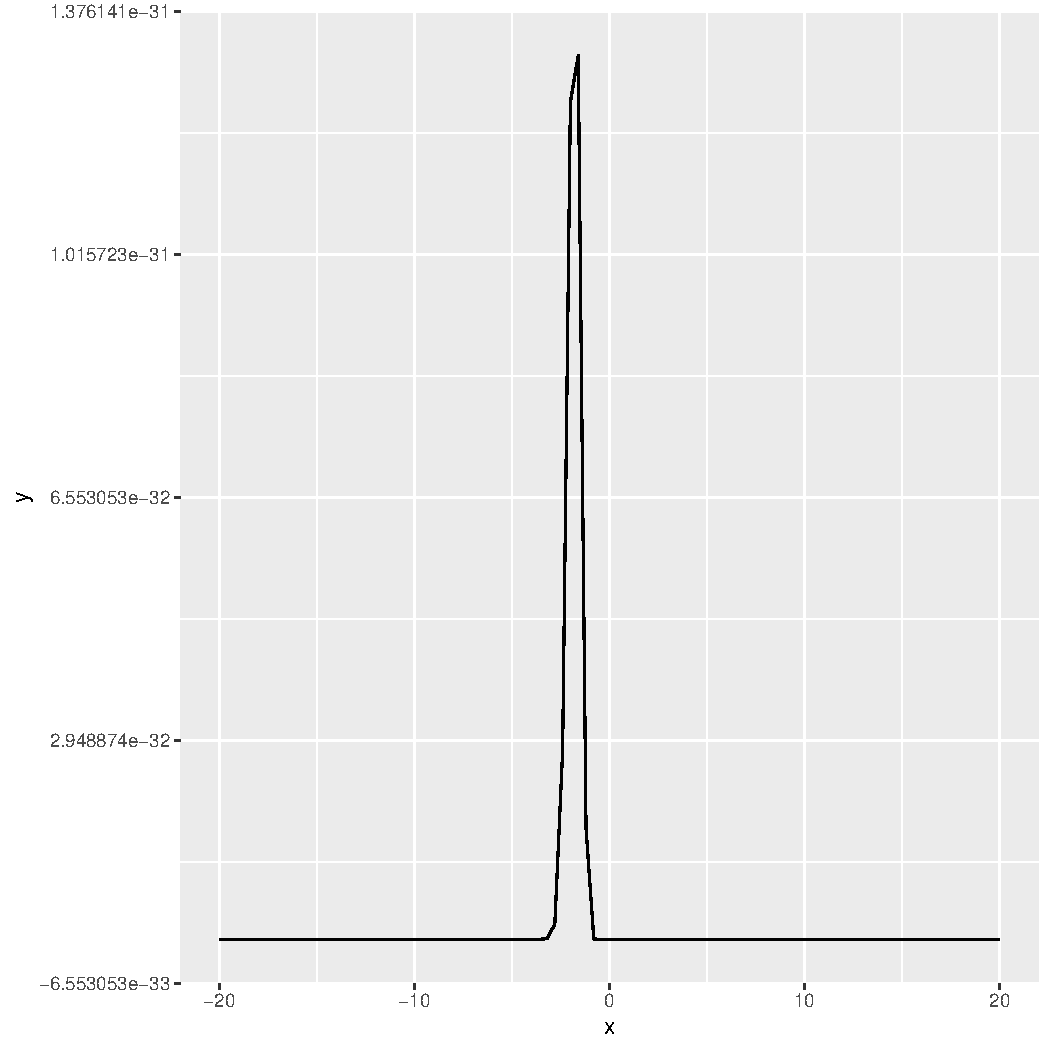
\includegraphics[width=\maxwidth]{figure/unnamed-chunk-2-1} 
\begin{kframe}\begin{alltt}
\hlcom{#clearly L is C_c(R) and we see that it spikes near 0, in (-10,10)}
\hldef{beta_1} \hlkwb{=} \hlkwd{optimise}\hldef{(L_1,} \hlkwd{c}\hldef{(}\hlopt{-}\hlnum{10}\hldef{,}\hlnum{10}\hldef{),}\hlkwc{maximum}\hldef{=}\hlnum{TRUE}\hldef{)}\hlopt{$}\hldef{maximum}
\hldef{beta_1}
\end{alltt}
\begin{verbatim}
## [1] -1.781288
\end{verbatim}
\end{kframe}
\end{knitrout}
			This is a good guess by MLE theory
\end{enumerate}
\item
	\begin{enumerate}[label=(\alph*)]
	\item
\begin{knitrout}
\definecolor{shadecolor}{rgb}{0.969, 0.969, 0.969}\color{fgcolor}\begin{kframe}
\begin{alltt}
        \hlcom{#clearly the function to plot is p(1-p)}
        \hldef{f_1} \hlkwb{=} \hlkwa{function}\hldef{(}\hlkwc{x}\hldef{) x}\hlopt{*}\hldef{(}\hlnum{1}\hlopt{-}\hldef{x)}
        \hlkwd{ggplot}\hldef{()}\hlopt{+}
        \hlkwd{geom_function}\hldef{(}\hlkwc{fun} \hldef{= f_1,} \hlkwc{xlim} \hldef{=} \hlkwd{c}\hldef{(}\hlopt{-}\hlnum{10}\hldef{,}\hlnum{10}\hldef{))}
\end{alltt}
\end{kframe}
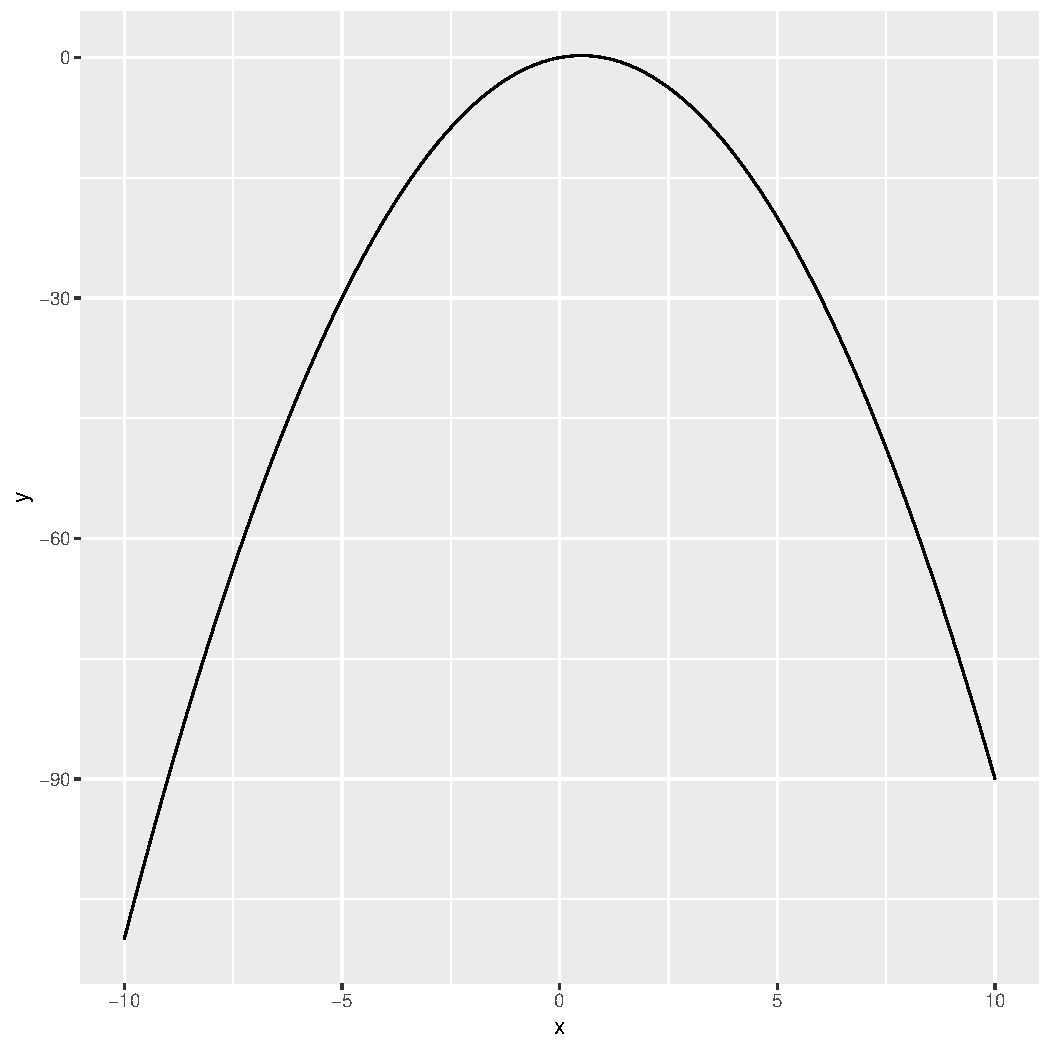
\includegraphics[width=\maxwidth]{figure/unnamed-chunk-3-1} 
\begin{kframe}\begin{alltt}
        \hlcom{#the maximum is}
        \hlkwd{optimise}\hldef{(f_1,} \hlkwd{c}\hldef{(}\hlopt{-}\hlnum{10}\hldef{,}\hlnum{10}\hldef{),}\hlkwc{maximum}\hldef{=}\hlnum{TRUE}\hldef{)}\hlopt{$}\hldef{maximum}
\end{alltt}
\begin{verbatim}
## [1] 0.5
\end{verbatim}
\end{kframe}
\end{knitrout}
	\item This probability is $p^{\sum_{i=1}^ny_i}(1-p)^{n-\sum_{i=1}^ny_i}$ as $Y_1,\ldots,Y_n\sim$ i.i.d. $\text{Bin}(1,p)$
	\item Here we clearly see that $L(p)=p^3(1-p)^2$
\begin{knitrout}
\definecolor{shadecolor}{rgb}{0.969, 0.969, 0.969}\color{fgcolor}\begin{kframe}
\begin{alltt}
\hldef{f_2} \hlkwb{=} \hlkwa{function}\hldef{(}\hlkwc{x}\hldef{) x}\hlopt{^}\hlnum{3} \hlopt{*} \hldef{(}\hlnum{1}\hlopt{-}\hldef{x)}\hlopt{^}\hlnum{2}
\hlkwd{plot}\hldef{(}\hlkwc{x}\hldef{=(}\hlnum{0}\hlopt{:}\hlnum{40}\hldef{)}\hlopt{/}\hlnum{40}\hldef{,} \hlkwc{y} \hldef{=} \hlkwd{f_2}\hldef{((}\hlnum{0}\hlopt{:}\hlnum{40}\hldef{)}\hlopt{/}\hlnum{40}\hldef{))}
\end{alltt}
\end{kframe}
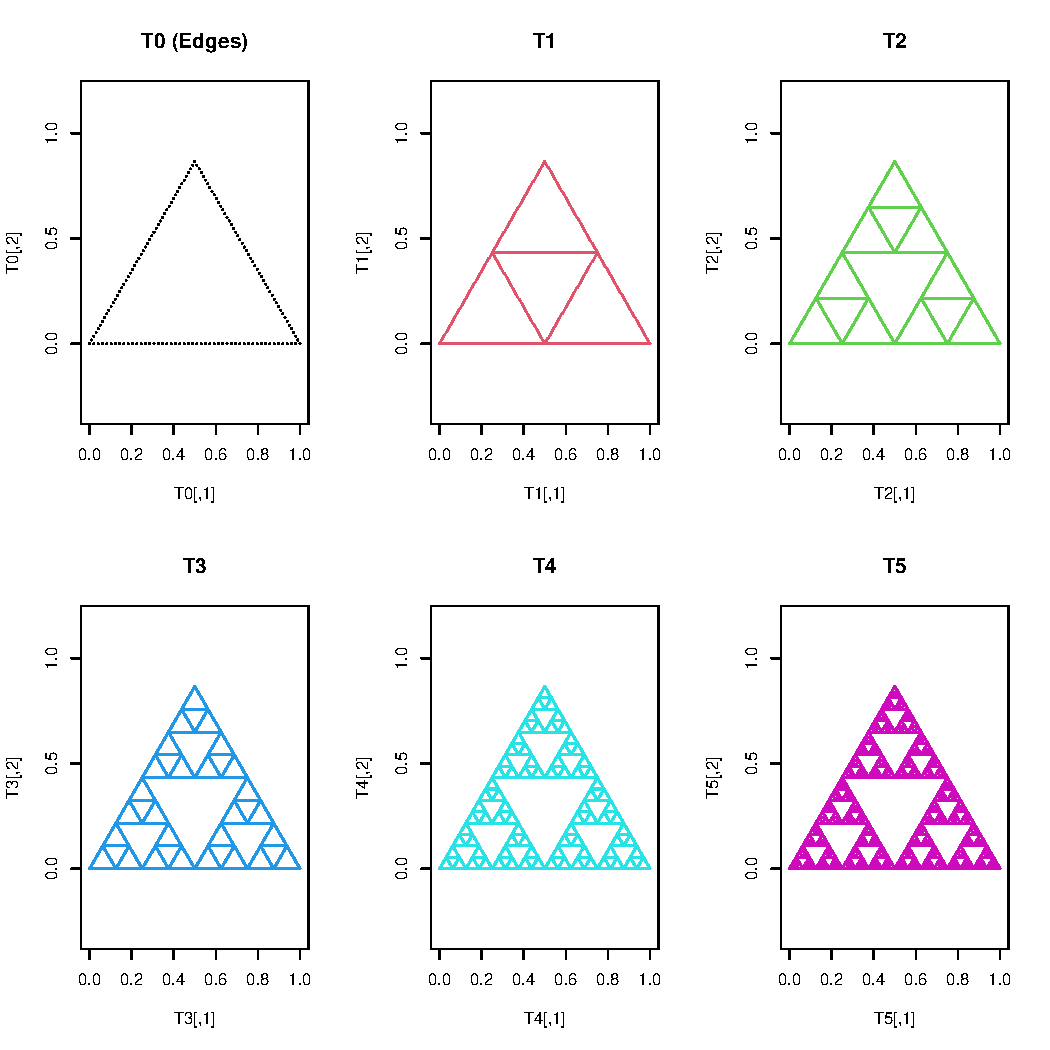
\includegraphics[width=\maxwidth]{figure/unnamed-chunk-4-1} 
\begin{kframe}\begin{alltt}
\hlkwd{plot}\hldef{(}\hlkwc{x}\hldef{=(}\hlnum{0}\hlopt{:}\hlnum{40}\hldef{)}\hlopt{/}\hlnum{40}\hldef{,} \hlkwc{y} \hldef{=} \hlkwd{log}\hldef{(}\hlkwd{f_2}\hldef{((}\hlnum{0}\hlopt{:}\hlnum{40}\hldef{)}\hlopt{/}\hlnum{40}\hldef{)))}
\end{alltt}
\end{kframe}
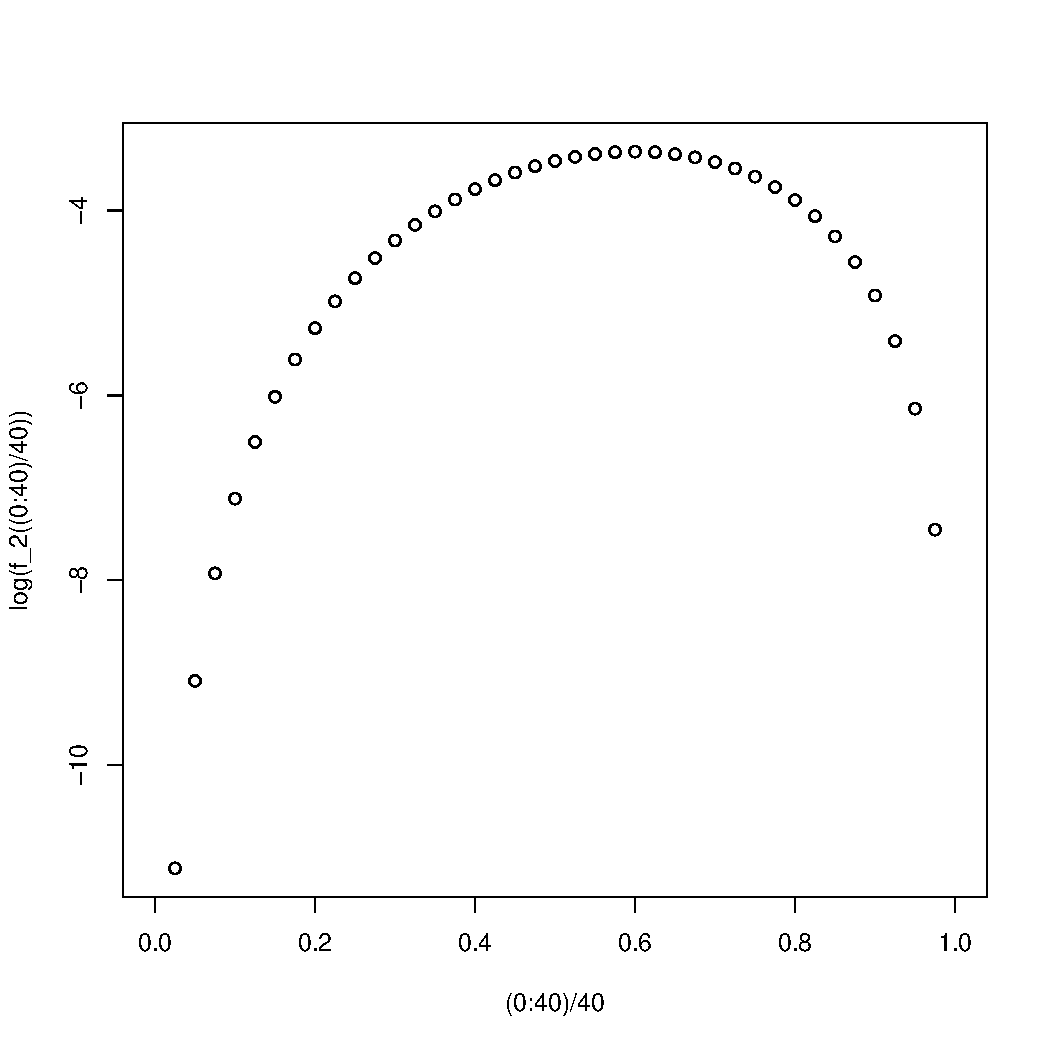
\includegraphics[width=\maxwidth]{figure/unnamed-chunk-4-2} 
\end{knitrout}
	\item
\begin{knitrout}
\definecolor{shadecolor}{rgb}{0.969, 0.969, 0.969}\color{fgcolor}\begin{kframe}
\begin{alltt}
\hlkwd{optimise}\hldef{(f_2,} \hlkwd{c}\hldef{(}\hlnum{0}\hldef{,}\hlnum{1}\hldef{),} \hlkwc{maximum}\hldef{=}\hlnum{TRUE}\hldef{)}\hlopt{$}\hldef{maximum}
\end{alltt}
\begin{verbatim}
## [1] 0.6000006
\end{verbatim}
\end{kframe}
\end{knitrout}
	\item $\hat{p}$ is a good guess for the actual value of $p$ that might result in such a result by MLE theory.
	\item
		\[
			\log\tilde{L}(\beta_0)=\log L(p)=\log\qty(p^{\sum y_i}(1-p)^{n-\sum y_i})=\log\qty(\qty( \frac{e^{\beta_0}}{1+e^{\beta_0}})^{\sum y_i}\qty( \frac{1}{1+e^{\beta_0}})^{n-\sum y_i})
		\]
		\[
			=\log\qty(e^{\beta_0\sum y_i}(1+e^{\beta_0})^{-n})=n\log\qty( \frac{1}{1+e^{\beta_0}})+\sum_{i=1}^n\beta_0y_i=\sum_{i=1}^n\qty(y_i\beta_0+\log\qty( \frac{1}{1+e^{\beta_0}}))
		\]
		We will proceed finding the \texttt{argmax} by maximising the log variant instead as $\log$ is a strictly increasing function on its domain. We will use the double derivative test
		\[
			\frac{d}{d\beta_0}\log\tilde{L}(\beta_0) = \sum_{i=1}^{n}y_i+n\frac{e^{\beta_0}}{(1+e^{\beta_0})}=0\implies \frac{e^{\beta_0}}{(1+e^{\beta_0})} = \frac{1}{n}\sum_{i=1}^ny_i
		\]
		\[
			\frac{d^2}{d\beta_0^2}\log\tilde{L}(\beta_0) = -n\qty( \frac{e^{\beta_0}}{(1+e^{\beta_0})^2})<0
		\]
		so by the double derivative rule there is unique maxima, achieved when the first derivative is $0$, solving that linear equation in $e^{\beta_0}$ and taking log gives,
		\[
			\hat{\beta_0}=\log\qty(\frac{\bar{y}}{1-\bar{y}})
		\]
		after some manipulation, where $\bar{y}=n^{-1}\sum_{i=1}^ny_i$
		\item It is $\log((3/5)/(1-(3/5)))=\log((3/5)/(2/5))=\log(3)-\log(2)$
\begin{knitrout}
\definecolor{shadecolor}{rgb}{0.969, 0.969, 0.969}\color{fgcolor}\begin{kframe}
\begin{alltt}
\hlkwd{log}\hldef{(}\hlnum{1.5}\hldef{)}
\end{alltt}
\begin{verbatim}
## [1] 0.4054651
\end{verbatim}
\end{kframe}
\end{knitrout}
			
		\item From the previous part,a good guess for $p$ here would be $\bar{y}=3/5$ so the probability for them to to win their next match would be (as the outcomes are independent), $p=3/5$
	\end{enumerate}
\item \begin{enumerate}[label=(\alph*)]
		\item by the previous problem we see that,
\begin{knitrout}
\definecolor{shadecolor}{rgb}{0.969, 0.969, 0.969}\color{fgcolor}\begin{kframe}
\begin{alltt}
\hldef{beta_0_hat} \hlkwb{=} \hlkwd{log}\hldef{((}\hlnum{724}\hlopt{/}\hlnum{2224}\hldef{)}\hlopt{/}\hldef{(}\hlnum{1}\hlopt{-}\hldef{(}\hlnum{724}\hlopt{/}\hlnum{2224}\hldef{)))}
\hldef{beta_0_hat}
\end{alltt}
\begin{verbatim}
## [1] -0.728429
\end{verbatim}
\end{kframe}
\end{knitrout}
		\item The probability of survival for any passenger is $724/2224$ which is
\begin{knitrout}
\definecolor{shadecolor}{rgb}{0.969, 0.969, 0.969}\color{fgcolor}\begin{kframe}
\begin{alltt}
\hlnum{724}\hlopt{/}\hlnum{2224}
\end{alltt}
\begin{verbatim}
## [1] 0.3255396
\end{verbatim}
\end{kframe}
\end{knitrout}
		\item The probability of death approximately $1-0.674=0.326<0.5$ so we can predict that this person likely died.
\end{enumerate}
\item \begin{enumerate}[label=(\alph*)]
		\item The lower levels (more depth) should correspond to lower fairs so we consider functions that map fare to depth and these have to be decreasing. Five examples of functions $f: \mathbb{R} \to [0,1]$ are:
		\begin{itemize}
			\item $f_1(x) = \frac{e^x}{1+e^x}$ 
			\item $f_2(x) = \Phi(x) \text{standard normal cdf}$ 
			\item $f_3(x) = \frac{1}{\pi}\arctan(x) + \frac{1}{2}$
			\item $f_4(x) = \frac{1}{2}\qty(1 + \text{erf}(x))$
			\item $f_5(x) = e^{-x^2}$
		\end{itemize}
		\item \begin{enumerate}[label=\roman*.]
			\item 
\begin{knitrout}
\definecolor{shadecolor}{rgb}{0.969, 0.969, 0.969}\color{fgcolor}\begin{kframe}
\begin{alltt}
\hldef{p_i} \hlkwb{=} \hlkwa{function}\hldef{(}\hlkwc{x}\hldef{,} \hlkwc{beta_1}\hldef{) \{} \hlkwd{exp}\hldef{(beta_1}\hlopt{*}\hldef{x)}\hlopt{/}\hldef{(}\hlnum{1}\hlopt{+}\hlkwd{exp}\hldef{(beta_1}\hlopt{*}\hldef{x)) \}}
\hlkwd{ggplot}\hldef{()} \hlopt{+}
\hlkwd{geom_function}\hldef{(}\hlkwc{fun} \hldef{=} \hlkwa{function}\hldef{(}\hlkwc{x}\hldef{)} \hlkwd{p_i}\hldef{(x,} \hlopt{-}\hlnum{1}\hldef{),} \hlkwd{aes}\hldef{(}\hlkwc{color} \hldef{=} \hlsng{"-1"}\hldef{),}
\hlkwc{xlim}\hldef{=}\hlkwd{c}\hldef{(}\hlopt{-}\hlnum{10}\hldef{,}\hlnum{10}\hldef{))} \hlopt{+}
\hlkwd{geom_function}\hldef{(}\hlkwc{fun} \hldef{=} \hlkwa{function}\hldef{(}\hlkwc{x}\hldef{)} \hlkwd{p_i}\hldef{(x,} \hlnum{0.5}\hldef{),} \hlkwd{aes}\hldef{(}\hlkwc{color} \hldef{=} \hlsng{"0.5"}\hldef{),}
\hlkwc{xlim}\hldef{=}\hlkwd{c}\hldef{(}\hlopt{-}\hlnum{10}\hldef{,}\hlnum{10}\hldef{))} \hlopt{+}
\hlkwd{geom_function}\hldef{(}\hlkwc{fun} \hldef{=} \hlkwa{function}\hldef{(}\hlkwc{x}\hldef{)} \hlkwd{p_i}\hldef{(x,} \hlnum{1}\hldef{),} \hlkwd{aes}\hldef{(}\hlkwc{color} \hldef{=} \hlsng{"1"}\hldef{),}
\hlkwc{xlim}\hldef{=}\hlkwd{c}\hldef{(}\hlopt{-}\hlnum{10}\hldef{,}\hlnum{10}\hldef{))} \hlopt{+}
\hlkwd{geom_function}\hldef{(}\hlkwc{fun} \hldef{=} \hlkwa{function}\hldef{(}\hlkwc{x}\hldef{)} \hlkwd{p_i}\hldef{(x,} \hlnum{10}\hldef{),} \hlkwd{aes}\hldef{(}\hlkwc{color} \hldef{=} \hlsng{"10"}\hldef{),}
\hlkwc{xlim}\hldef{=}\hlkwd{c}\hldef{(}\hlopt{-}\hlnum{10}\hldef{,}\hlnum{10}\hldef{))} \hlopt{+}
\hlkwd{labs}\hldef{(}\hlkwc{color} \hldef{=} \hlsng{"beta_1"}\hldef{,} \hlkwc{x} \hldef{=} \hlsng{"x_i"}\hldef{,} \hlkwc{y} \hldef{=} \hlsng{"p_i"}\hldef{)}
\end{alltt}
\end{kframe}
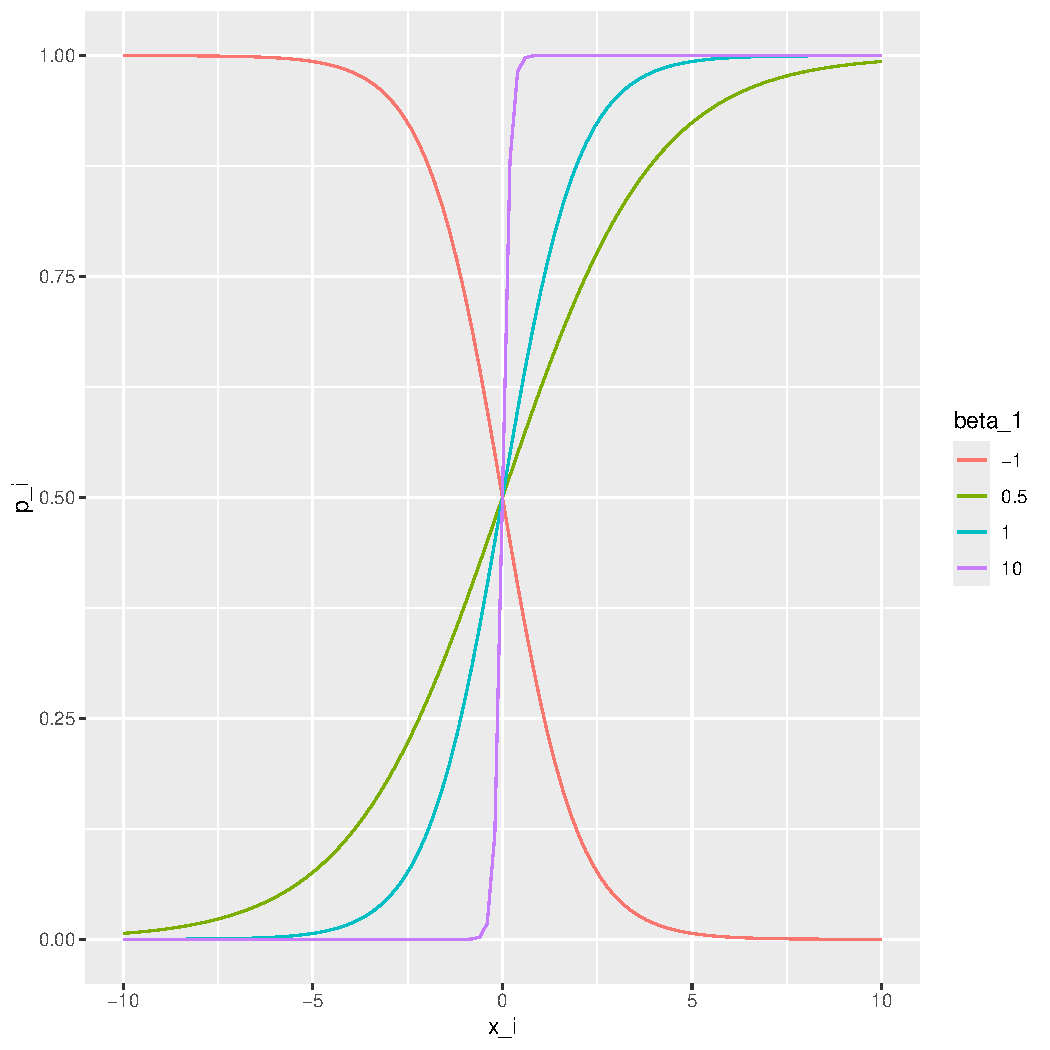
\includegraphics[width=\maxwidth]{figure/unnamed-chunk-9-1} 
\end{knitrout}
			\item The function $p_i(x_i)$ is an increasing function of $x_i$ when $\beta_1 > 0$. An increasing function implies that as the fare ($x_i$) increases, the probability of survival ($p_i$) also increases. Conversely, a decreasing function (when $\beta_1 < 0$) implies that paying a higher fare corresponds to a lower probability of survival.
			\item When $x_i = 0$, $p_i = \frac{e^0}{1+e^0} = \frac{1}{2} = 0.5$. This seems too high for the Titanic data. Since the overall baseline survival rate was much lower (approximately $32.55\%$), a fare of $0$ (representing the poorest passengers or crew members) should correspond to a survival probability significantly lower than the average.
			\item We can modify the function by adding an intercept term $\beta_0$ to the exponent:
			\[
				p_i(x_i) = \frac{e^{\beta_0 + \beta_1 x_i}}{1 + e^{\beta_0 + \beta_1 x_i}}
			\]
		\end{enumerate}
		\item Using the modified function from part (b)iv, the likelihood function is the product of the probabilities of the observed independent outcomes:
		\[
			L(\beta_0, \beta_1) = \prod_{i=1}^n p_i(x_i)^{y_i} (1-p_i(x_i))^{1-y_i} = \prod_{i=1}^n \qty( \frac{e^{\beta_0 + \beta_1 x_i}}{1 + e^{\beta_0 + \beta_1 x_i}} )^{y_i} \qty( \frac{1}{1 + e^{\beta_0 + \beta_1 x_i}} )^{1-y_i}
		\]
		\item We can use Maximum Likelihood Estimation (MLE). By taking the natural logarithm of the likelihood function to obtain the log-likelihood $\log L(\beta_0, \beta_1)$, we can compute its partial derivatives with respect to $\beta_0$ and $\beta_1$. Setting these partial derivatives to $0$ gives a system of equations. Solving this system (typically using numerical optimization algorithms like \texttt{optimise} in R) will yield the estimates $(\hat{\beta}_0, \hat{\beta}_1)$ that maximize the likelihood of observing our data.
\end{enumerate}
\end{enumerate}
\end{document}
